\documentclass[border=8pt]{standalone}
\usepackage[utf8]{inputenc}
\usepackage{tikz}
\usetikzlibrary{positioning, arrows.meta}

\tikzset{
  entita/.style = {rectangle, draw, thick, fill=blue!8, minimum width=30mm, minimum height=14mm, font=\small},
  subent/.style = {rectangle, draw, thick, fill=blue!8, minimum width=38mm, minimum height=11mm, font=\small},
  attr/.style   = {circle, draw, thick, fill=white, minimum size=5pt, inner sep=0},
  pk/.style     = {circle, draw, thick, fill=black, minimum size=5pt, inner sep=0},
  link/.style   = {thick},
  isa/.style    = {thick, -{Triangle[open]}},
  et/.style     = {font=\footnotesize}
}

\begin{document}
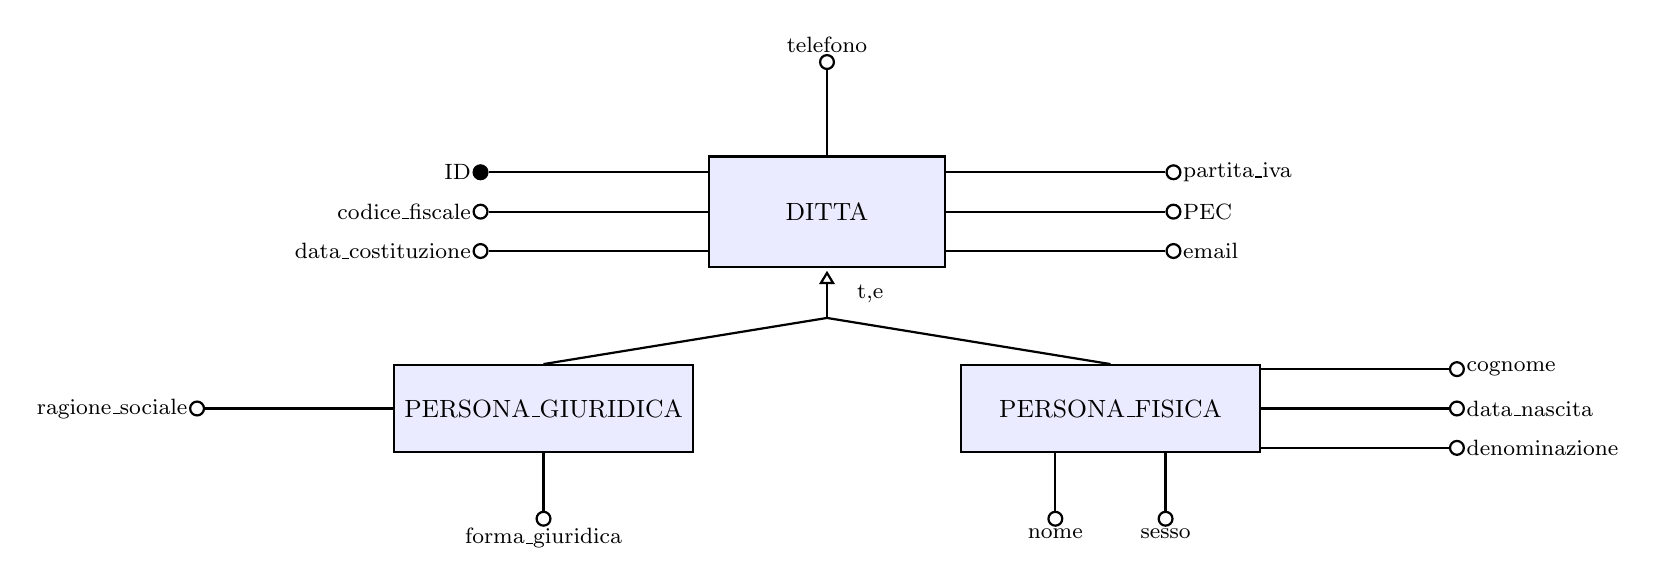
\begin{tikzpicture}

  % ---------- DITTA (padre) ----------
  \node[entita] (D) at (0,3.5) {DITTA};

  \node[pk]   (id)  at (-4.4,4.0){}; \draw[link] (-1.5,4.0)--(id);  \node[et,left] at (id)  {ID};
  \node[attr] (cf)  at (-4.4,3.5){}; \draw[link] (-1.5,3.5)--(cf);  \node[et,left] at (cf)  {codice\_fiscale};
  \node[attr] (dco) at (-4.4,3.0){}; \draw[link] (-1.5,3.0)--(dco); \node[et,left] at (dco) {data\_costituzione};

  \node[attr] (piva) at (4.4,4.0){}; \draw[link] (1.5,4.0)--(piva); \node[et,right] at (piva) {partita\_iva};
  \node[attr] (pec)  at (4.4,3.5){}; \draw[link] (1.5,3.5)--(pec);  \node[et,right] at (pec)  {PEC};
  \node[attr] (em)   at (4.4,3.0){}; \draw[link] (1.5,3.0)--(em);   \node[et,right] at (em)   {email};

  \node[attr] (tel) at (0,5.4){}; \draw[link] (0,4.2)--(tel); \node[et,above] at (tel) {telefono};

  % ---------- generalizzazione (totale, esclusiva) ----------
  \node[subent] (PG) at (-3.6,1.0) {PERSONA\_GIURIDICA};
  \node[subent] (PF) at ( 3.6,1.0) {PERSONA\_FISICA};
  \coordinate (fork) at (0,2.15);
  \draw[isa] (fork) -- (0,2.75);              % is-a verso il padre
  \draw[link] (PG.north) -- (fork);
  \draw[link] (PF.north) -- (fork);
  \node[et] at (0.55,2.45) {t,e};

  % attributi PERSONA_GIURIDICA
  \node[attr] (rs) at (-8.0,1.0){}; \draw[link] (-5.5,1.0)--(rs); \node[et,left] at (rs) {ragione\_sociale};
  \node[attr] (fg) at (-3.6,-0.4){}; \draw[link] (-3.6,0.45)--(fg); \node[et,below] at (fg) {forma\_giuridica};

  % attributi PERSONA_FISICA
  \node[attr] (cog) at (8.0,1.5){}; \draw[link] (5.5,1.5)--(cog); \node[et,right] at (cog) {cognome};
  \node[attr] (dn)  at (8.0,1.0){}; \draw[link] (5.5,1.0)--(dn);  \node[et,right] at (dn)  {data\_nascita};
  \node[attr] (den) at (8.0,0.5){}; \draw[link] (5.5,0.5)--(den); \node[et,right] at (den) {denominazione};
  \node[attr] (nom) at (2.9,-0.4){}; \draw[link] (2.9,0.45)--(nom); \node[et,below] at (nom) {nome};
  \node[attr] (ses) at (4.3,-0.4){}; \draw[link] (4.3,0.45)--(ses); \node[et,below] at (ses) {sesso};

\end{tikzpicture}
\end{document}
